% !TEX root = rampMeteringViaTheAdjoint.tex
\label{sec:contBufferModel}
\subsection{Weak boundary conditions and ramp flux demands}

One condition we wish our continuous model to possess is mass-conservation
on the ramp demands. In other words, for a ramp at cell $\icell$,
we want the demand at the ramp to apply to the system in a \emph{strong}
sense. For horizontal queues with density having a spacial and temporal
dependency, backwards-moving shocks could cause a density boundary
condition to not apply, thus \emph{weak} boundary conditions are considered
for these models. Then, the flux at such a boundary condition would
be determined from the solution of a junction problem at the weak boundary
condition. Let $\totalrampflow{\icell}t$ be the boundary flow specification,
and let $\actualrampflow{\icell}t$ be the actual boundary flux. Then
our condition amounts to:

\begin{equation}
\int_{t=0}^{\ntime}\totalrampflow{\icell}tdt=\int_{t=0}^{\ntime}\actualrampflow{\icell}tdt\label{eq:condition1}
\end{equation}


For the horizontal queueing model, we have:

\[
\actualrampflow{\icell}t=f_{i}(\hat{\densitysymbol}\left(f_{\icell}^{-1,\text{ff}}\left(\totalrampflow{\icell}t\right),\density{\icell}{a_{i},t}\right)\le\totalrampflow{\icell}t
\]


where $f\left(\cdot\right)$ is the flux function mapping density
to flux, $f_{\icell}^{-1,\text{ff}}\left(\totalrampflow{\icell}t\right)$
is the inverse mapping of flux to the corresponding free-flow density,
$\densitysymbol_{\icell}\left(a_{i},t\right)$ is the density at the
beginning of cell $\icell$ at time $t$, and $\hat{\densitysymbol}$
is the solution of the Riemann problem at the boundary. The solution
of $\hat{\densitysymbol}$ admits fluxes that can be strictly less
than $\totalrampflow{\icell}t$, but never greater than $\totalrampflow{\icell}t$.
If this limiting flux condition occurs over a time period $\left[t_{1},t_{2}\right]$,
then Equation~(\ref{eq:condition1}) becomes:

\begin{eqnarray}
\int_{t=\bar{t_{1}}}^{\bar{t_{2}}}\actualrampflow{\icell}tdt & \le\int_{t=\bar{t_{1}}}^{\bar{t_{2}}}\totalrampflow{\icell}t & \forall\mbox{\ensuremath{\bar{t_{1}}\le\bar{t_{2}}}},\\
\int_{t=t_{1}}^{t_{2}}\actualrampflow{\icell}tdt & <\int_{t=t_{1}}^{t_{2}}\totalrampflow{\icell}tdt & \implies\\
\int_{t=0}^{T}\actualrampflow{\icell}tdt & <\int_{t=0}^{T}\totalrampflow{\icell}tdt
\end{eqnarray}


This shows that having a horizontal queue model for the onramp will
not guarantee a strong application of flux boundary conditions.


\subsection{Buffer model for ramps\label{sub:Buffer-model-for}}

To overcome this shortcoming on ramps, we propose to use a \emph{buffer}
ODE for the ramp model, and have the ODE interact with the larger
PDE system via the junction model. For a ramp at cell $\icell$, let
the ODE of queue length $\rampqueue{\icell}t$ be:

\begin{equation}
\frac{d\rampqueue{\icell}t}{dt}=\totalrampflow{\icell}t-\rampflux{\icell}t\label{eq:rampode}
\end{equation}


where $\gamma$ denotes the outgoing flux from the ramp. It is obvious from this model
that the inflow into the ramp will be equal to the condition specified
in Equation~(\ref{eq:condition1}).

For the junction model, we solve for the fluxes across junctions by
maximizing the flow across a junction given the demands of the incoming
links and the supplies of the outgoing links. The mainline links determine
their demands and supplies as done in~\cite{garavello2006traffic}. The
onramp demand is given by the following equation:

\[
\rampdemand{\icell}t=\begin{cases}
\maxrampflux{\icell} & \rampqueue{\icell}t>0\\
\totalrampflow{\icell}t & \text{otherwise}
\end{cases}
\]


which permits the physically allowable flux out of the ramp when there
is a queue, and the current input flux of the buffer otherwise. Finally,
the offramp should be considered to have infinite supply.

The linear program will solve for three relevant fluxes: $\flux{\icell}t,\rampflux{\icell}t,$
and $\flux{\icell+1}t$ which represent the flux from the current
cell into the junction, the flux out of the ramp, and the flux out
of the junction into the downstream cell respectively. The boundary
densities, $\hat{\densitysymbol}$, for the mainlines would be determined
as in \cite{garavello2006traffic}. The following system would constitute
a full solution of the junction problem, and would also determine
the ramp flux $\rampflux{\icell}t$ necessary to virtualSelfthe ramp virtualSelfSimilarE
in Equation~(\ref{eq:rampode}).


\subsection{Unique and self-similar solutions for the continuous model}


% \subsubsection{Virtual Junction Problem Approach}\label{sub:bestselfsimilar}
% % !TEX root = rampMeteringViaTheAdjoint.tex
\begin{figure}
	\centering
	\begin{displaymath}
    \xymatrix{ \bullet \ar[r]| {\linkmlone} & \bullet   \ar[r]| {\linkmltwo} \ar[dr]| {\linkoff} & \bullet  \\
			    \ar[ur]|{\linkon}  &   &  }
\end{displaymath}
	\caption{Illustration of junction under consideration}
	\label{fig:contJuncIll}
\end{figure}
Reference Figure~\ref{fig:contJuncIll} for the notation used in the current junction problem. Let $\fluxsymbol, \densitysymbol$ be the vector notation for fluxes and densities on the links respectively. Let the ($\rsind{}$) notation denote variables pertaining to a Riemann solution, and let the ($\virtualind{}$) notation denote variables pertaining to the \emph{virtual} junction problem. Let $\maxflux_i$ denote the maximum flux allowed from or into a link $i$, depending on the context. For instance, $\virtualind{\rsind{\maxflux}}_{\linkmltwo}$ would be the maximum flux allowed into link $\linkmltwo$ for the virtual junction problem, considering the state given from the Riemann solution of the initial data $\densitysymbol$.

Define the mapping from densities and ramp queues to maximum flux as $\feasibleflux \left(\densitysymbol, \rampqueuesymbol_{\linkon}, \rampcontrolsymbol_{\linkon} \right) = \maxflux$, where the maximum fluxes are determined as in Section~\ref{sec:problemFormulation}.

Define the mapping from our maximum fluxes $\maxflux$ to a ``virtual''
flux $\virtualind{\maxflux}$:

\[
\virtualind{\maxflux}_{i}=\virtualmap{\maxflux_{i},\offrampratiosymbol}=\begin{cases}
\left(1-\offrampratiosymbol\right)\maxflux_{i} & i=\linkmlone\\
\maxflux_{i} & \text{o.w.}
\end{cases}
\]


Define the virtual junction flux solver as $\jsvirt{\virtualind{\maxflux},\prioritysymbol}=\virtualind{\fluxsymbol}$,
which takes the virtual demands from the incoming mainline and ramp
and the supply of the outgoing mainline, as well as a priority factor
$\prioritysymbol$, and produces resultant fluxes $\virtualind{\fluxsymbol}$
by applying the flow maximization criteria across a 2-to-1 merge model
of \cite{garavello2006traffic}. 
\begin{lem}
\label{lem:max-flow-js}$\sum\jsvirt{\virtualind{\maxflux},\prioritysymbol}=2\left(\min\left(\maxflux_{\linkmlone}\left(1-\beta\right)+\maxflux_{\linkon},\maxflux_{\linkmltwo}\right)\right)$\end{lem}
\begin{proof}
Result of flow maximization criteria and the virtual mapping $\virtualmap{}$.
\end{proof}
Let the limiting side, $\limitingside$ ($\negate{\limitingside}$
being the complement), being either \emph{demand-limited} ($\demandlimited$) or \emph{supply-limited} ($\supplylimited$), be defined
by:

\[
\limitingside\left(\maxflux\right)=\begin{cases}
\demandlimited & \maxflux_{\linkmltwo}<\maxflux_{\linkmlone}\left(1-\beta\right)+\maxflux_{\linkon}\\
\supplylimited & \text{otherwise}
\end{cases}
\]


The definition is modified for the virtual problem to be:

\[
\virtualind{\limitingside}\left(\virtualind{\maxflux}\right)=\begin{cases}
\demandlimited & \virtualind{\maxflux}_{\linkmltwo}<\virtualind{\maxflux}_{\linkmlone}+\virtualind{\maxflux}_{\linkon}\\
\supplylimited & \text{otherwise}
\end{cases}
\]

\begin{lem}
\label{lem:lsprime-equals-ls-1}$\limitingside\left(\maxflux\right)=\virtualind{\limitingside}\left(\virtualmap{\maxflux}\right)$\end{lem}
\begin{proof}
From the $\limitingside,\virtualind{\limitingside}$ definitions and
the definition of the virtual map $\virtualmap{}$.
\end{proof}
Define the mapping from initial density $\densitysymbol$ and resultant
flux $\fluxsymbol$ to link-boundary density $\rsind{\densitysymbol}$
as $\rsinrhomap{\fluxsymbol,\densitysymbol}$ or $\rsoutrhomap{\fluxsymbol,\densitysymbol}$,
and let these definitions match \cite{garavello2006traffic}.

We can now define or Riemann solver $\RS{\densitysymbol_{\linkmlone},\densitysymbol_{\linkmltwo},\rampqueuesymbol_{\linkon},\rampcontrolsymbol,\offrampratiosymbol,\priority{},\totalrampflowsymbol}=\left(\rsind{\densitysymbol}_{\linkmlone},\rsind{\densitysymbol}_{\linkmltwo},\fluxsymbol_{\linkon} \right)$.
Determined by the following process:
\begin{enumerate}
\item Determine demands and supplies $\maxflux = \feasibleflux \left(\densitysymbol, \rampqueuesymbol, \rampcontrolsymbol \right)$ for the mainlines and ramp.
\item Map to virtual fluxes $\virtualind{\maxflux}=\virtualmap{\maxflux}$
\item Apply the virtual junction solver $\virtualind{\fluxsymbol}=\jsvirt{\virtualind{\maxflux}}$
\item Map back to standard fluxes $\fluxsymbol=\invvirtualmap{\virtualind{\fluxsymbol}}$
\item Solve for boundary densities $\rsinrhomap{\fluxsymbol_{\linkmlone},\densitysymbol_{\linkmlone}}$,
$\rsoutrhomap{\fluxsymbol_{\linkmltwo},\densitysymbol_{\linkmltwo}}$,
ramp flow $\fluxsymbol_{\linkon}$ and offramp flow $\offrampratiosymbol\fluxsymbol_{\linkmlone}$
\end{enumerate}
Existence and uniqueness of the outputs of $\RS{\cdot}$ are given
by the existence and uniqueness of our virtual mapping functions $\virtualmap{\cdot},\invvirtualmap{\cdot}$
and the results of~\cite{garavello2006traffic}. The density profile
solution is also admissible in the sense of \cite{garavello2006traffic},
as the split ratio matrix is satisfied, there is flow conservation
across the junction (Rankine-Huginiot condition at junctions), and
the density profiles within cells are consistent with the weak solution
of the LWR equation. What we have left to show is that our Riemann
solver is self-similar, or more specifically:

\[
\RS{\rsind{\densitysymbol}_{\linkmlone},\rsind{\densitysymbol}_{\linkmltwo},\rampqueuesymbol_{\linkon},\rampcontrolsymbol,\offrampratiosymbol,\priority{},\totalrampflowsymbol}=\RS{\densitysymbol_{\linkmlone},\densitysymbol_{\linkmltwo},\rampqueuesymbol_{\linkon},\rampcontrolsymbol,\offrampratiosymbol,\priority{},\totalrampflowsymbol}=\left(\rsind{\densitysymbol}_{\linkmlone},\rsind{\densitysymbol}_{\linkmltwo},\fluxsymbol_{\linkon}\right)
\]


We note that the onramp's demand is the same for both expressions
above and it uses the $\fluxsymbol_{\linkon}$ value to updates its
queue length $\rampqueuesymbol$:

\[
\dot{\rampqueuesymbol}=\totalrampflowsymbol-\fluxsymbol_{\linkon}
\]


To show the self-similar property, we show that we can equivalently
demonstrate that the virtual flux out of link $\linkmlone$ is self-similar
in the virtual junction solver $\jsvirt{\cdot}$. 
\begin{lem}
\label{lem:maxed-flux}$\fluxsymbol=\maxflux\implies\rsind{\feasibleflux}=\feasibleflux$, 
\end{lem}

\begin{lem}
\label{lem:supset-ls-not}$\rsind{\feasibleflux}_{\negate{\limitingside}}\supseteq\feasibleflux_{\negate{\limitingside}}$
\end{lem}

\begin{lem}
\label{lem:supset-ls}$\rsind{\feasibleflux}_{\limitingside}=\feasibleflux_{\limitingside}$\end{lem}
\begin{proof}
From definition of $\rsinrhomap{\fluxsymbol,\densitysymbol}$ and
$\rsoutrhomap{\fluxsymbol,\densitysymbol}$.\end{proof}
\begin{lem}
\label{lem:ls-rs-equals-ls}$\rsind{\virtualind{\limitingside}}=\virtualind{\limitingside}$\end{lem}
\begin{proof}
From Lemmas~\ref{lem:supset-ls-not}, \ref{lem:supset-ls}\end{proof}
\begin{lem}
$\rsind{\virtualind{\fluxsymbol}}_{\linkmltwo}=\virtualind{\fluxsymbol}_{\linkmltwo}$\label{lem:equal-flux-two}\end{lem}
\begin{proof}
From Lemma~\ref{lem:supset-ls}, \ref{lem:ls-rs-equals-ls} and
flow maximization in Lemma~\ref{lem:max-flow-js}, we have that the
total flux across the junction for the Riemann solution is identical
to the initial problem.\end{proof}
\begin{lem}
\label{lem:match-flux-virtual}If \textup{$\rsind{\virtualind{\fluxsymbol}}_{\linkmlone}=\virtualind{\fluxsymbol}_{\linkmlone}$,
then $\RS{\cdot}$ is self-similar.}\end{lem}
\begin{proof}
From Lemma~\ref{lem:equal-flux-two}, we have $\rsind{\virtualind{\fluxsymbol}}_{\linkmlone}=\virtualind{\fluxsymbol}_{\linkmlone}\implies\rsind{\virtualind{\fluxsymbol}}=\virtualind{\fluxsymbol}$. Clearly, $\rsind{\rsind{\fluxsymbol}}_{\linkon} = \rsind{\fluxsymbol}_{\linkon}$.
Now we show show $\rsind{\virtualind{\fluxsymbol}}=\virtualind{\fluxsymbol}$
implies the Riemann solver is self-similar. The $\rsind{\densitysymbol}$
solutions have the property that $\rsind{\densitysymbol}\left(\fnflux{\rsind{\densitysymbol}},\rsind{\densitysymbol}\right)=\rsind{\densitysymbol}$,
and $\fnflux{\rsind{\densitysymbol}}=\fluxsymbol$. From the uniqueness
of the inverse virtual mapping $\invvirtualmap{\cdot}$, $\rsind{\virtualind{\fluxsymbol}}=\virtualind{\fluxsymbol}\implies\rsind{\fluxsymbol}=\fluxsymbol$. Therefore,
\begin{align}
\virtualind{\rsind{\fluxsymbol}} = \virtualind{\fluxsymbol} & \implies \\
\rsind{\fluxsymbol} = \fluxsymbol & \implies \\
\rsind{\densitysymbol}\left(\rsind{\fluxsymbol},\rsind{\densitysymbol} \right) = 
\rsind{\densitysymbol}\left(\fluxsymbol,\rsind{\densitysymbol} \right) = 
\rsind{\densitysymbol}\left(\fnflux{\rsind{\densitysymbol}},\rsind{\densitysymbol} \right) =
\rsind{\densitysymbol}
\end{align}
\end{proof}
\begin{thm}
\textup{\label{thm:one-equals-one}$\RS{\cdot}$ is self-similar.}
\end{thm}
We need to show $\rsind{\virtualind{\fluxsymbol}}_{\linkmlone}=\virtualind{\fluxsymbol}_{\linkmlone}$.
When the problem is demand-limited, it is obvious using Lemmas~\ref{lem:supset-ls}
and \ref{lem:ls-rs-equals-ls}. When the problem is supply-limited,
we give some properties. The virtual incoming fluxes are determined
by $\jsvirt{\cdot}$ by minimizing the Euclidean distance of $\left(\fluxsymbol_{\linkmlone,}\fluxsymbol_{\linkon,}\right)$
from $\left(\prioritysymbol\maxflux_{\linkmltwo},\maxflux_{\fluxsymbol}-\prioritysymbol\maxflux_{\linkmltwo}\right)$
such that $\left(\fluxsymbol_{\linkmlone,}\fluxsymbol_{\linkon,}\right)$
is feasible. Note that the reference point $\left(\prioritysymbol\maxflux_{\linkmltwo},\maxflux_{\fluxsymbol}-\prioritysymbol\maxflux_{\linkmltwo}\right)$
will not change with assumption of being supply-limited. Additionally,
Lemma~\ref{lem:supset-ls-not} tells us the feasible set of $\left(\fluxsymbol_{\linkmlone,}\fluxsymbol_{\linkon,}\right)$
only increases.

We consider the case when $\fluxsymbol_{\linkmlone}<\maxflux_{\linkmlone},\fluxsymbol_{\linkon}<\maxflux_{\linkon},$
and otherwise. For the first case, the reference point is feasible,
and thus reference point will be optimal for both the original and
final problem.

Otherwise, one of the incoming links $i$ is at $\maxflux_{i}$, and
the optimal point of the initial problem resides on the boundary of
the feasible region. Lemma~\ref{lem:maxed-flux} tells us the maxed
link's demand will not change. Combined with the fact that the feasible
region of the demands for the virtual junction problem in the Riemann
solution $\left(\maxflux'_{\linkmlone},\maxflux'_{\linkon}\right)$
only increases (from Lemma~\ref{lem:supset-ls-not}), the optimal
point of the junction problem will remain at the same boundary point.

For all cases, we have demonstrated $\virtualind{\fluxsymbol}_{\linkmlone}=\fluxsymbol_{\linkmlone}$,
thus completing the proof. See Figure~\ref{fig:virtualSSFigure} for an illustration of this proof.

\begin{figure}[h]
\centering
\subfloat[Interior Example]{
\resizebox{.5\columnwidth}{!}{
	\def \rampDem{1.8}
\def \dem{2.5}
\def \priorityRat{0.55}
\def \totalFlow{3.2}
\def \twoGap{.5}
\def \twoGapDem{.3}


\begin{tikzpicture}[scale=\scale,domain=0:1]

\coordinate (Z) at (0,0);
\coordinate (I1) at (\rampDem, 0);
\coordinate (I2) at (0, \dem);
\coordinate (I3) at (\rampDem, \dem);
\coordinate (I4) at (\rampDem+\twoGap, 0);
\coordinate (I5) at (\rampDem+\twoGap, \dem);
\coordinate (I6) at (0, \dem+\twoGapDem);
\coordinate (I7) at (\rampDem+\twoGap, \dem+\twoGapDem);
\coordinate (I8) at (\rampDem, \dem+\twoGapDem);
\coordinate (A) at (0, {\totalFlow});
\coordinate (B) at (\totalFlow, 0);
\coordinate (C) at ({(1-\priorityRat)/\priorityRat*\dem}, \dem+\twoGapDem);
\coordinate (P1) at (intersection of I1--I3 and A--B);
\coordinate (P2) at (intersection of I2--I3 and A--B);


\draw[->] (Z) -- (4,0) node[below right]{$\gamma_{1,0^+}$};
\draw[->] (Z) -- (0,4) node[left]{$\gamma_{r,0^+}$};
\draw[dashed] (I8) -- (I1) node[below]{$\beta\gamma^{\max}_{1,0}$};
\draw[dashed, line width = 2pt] (I7) -- (I4) node[below]{$\beta\gamma^{\max}_{1,0^+}$};
\draw[dashed] (I5) -- (I2) node[left]{$\gamma^{\max}_{r,0}$};
\draw[dashed, line width = 2pt] (I7) -- (I6) node[left]{$\gamma^{\max}_{r,0^+}$};
\draw (A) -- (B) node{};
\draw[->] (Z) -- (C) node[above, xshift=1cm]{};
\draw[color=red, line width = 2pt] (intersection of A--B and Z--C) node[left] {Optimal} circle (1pt);


\end{tikzpicture}
}
\label{fig:virtualSSInterior}
}
\subfloat[Boundary Example]{
\resizebox{.5\columnwidth}{!}{
	% !TEX root = rampMeteringViaTheAdjoint.tex
\def \rampDem{1.7}
\def \dem{1.5}
\def \priorityRat{0.8}
\def \totalFlow{2.5}
\def \twoGap{.3}

\begin{tikzpicture}[scale=\scale,domain=0:1]

\coordinate (Z) at (0,0);
\coordinate (I1) at (\rampDem, 0);
\coordinate (I2) at (0, \dem);
\coordinate (I3) at (\rampDem, \dem);
\coordinate (I4) at (\rampDem+\twoGap, 0);
\coordinate (I5) at (\rampDem+\twoGap, \dem);
\coordinate (A) at (0, {\totalFlow});
\coordinate (B) at (\totalFlow, 0);
\coordinate (C) at ({(1-\priorityRat)/\priorityRat*\dem}, \dem);
\coordinate (Cplus) at ({(1-\priorityRat)/\priorityRat*\totalFlow}, \totalFlow);
\coordinate (P1) at (intersection of I1--I3 and A--B);
\coordinate (P2) at (intersection of I2--I3 and A--B);


\draw[->] (Z) -- (3,0) node[below right]{$\rsind{\virtualind{\fluxsymbol_{\linkmlone}}}$};
\draw[->] (Z) -- (0,3) node[left]{$\rsind{\virtualind{\fluxsymbol_{\linkon}}}$};
\draw[dashed] (I3) -- (I1) node[below]{$\virtualind{\maxflux_{\linkmlone}}$};
\draw[dashed, line width = 2pt] (I5) -- (I4) node[below]{$\virtualind{\rsind{\maxflux}}_{\linkmlone}$};
\draw[dashed, line width = 2pt] (I5) -- (I2) node[left]{$\virtualind{\rsind{\maxflux}}_{\linkon},\virtualind{\maxflux_{\linkon}}$};
\draw (A) -- (B) node[yshift=1cm, xshift=0cm]{$\rsind{\virtualind{\fluxsymbol_{\linkon}}}+\rsind{\virtualind{\fluxsymbol_{\linkmlone}}}=\virtualind{\rsind{\maxflux}}_{\linkmltwo}$};
\draw (Z) -- (C) node[below, xshift=1cm,yshift=-1cm,]{$\rsind{\virtualind{\fluxsymbol_{\linkmlone}}}=\left(\frac{\prioritysymbol}{1-\prioritysymbol}\right)\rsind{\virtualind{\fluxsymbol_{\linkon}}}$};
\draw[dashed,->] (C) -- (Cplus);
\draw (intersection of A--B and Z--C) node [right](xseclabel){$\left(\prioritysymbol\maxflux_{\linkmltwo},\maxflux_{\fluxsymbol}-\prioritysymbol\maxflux_{\linkmltwo}\right)$} circle (1pt);
\draw[color=red, line width = 2pt] (intersection of I5--I2 and A--B) node[above,xshift=1cm] (optimallabel){Optimal} circle (1pt);

\end{tikzpicture}

}
\label{fig:virtualSSBoundary}
}
\caption{Illustration of Theorem~\ref{thm:one-equals-one}}
\label{fig:virtualSSFigure}
\end{figure}


% \subsubsection{Old Approach}\label{sub:oldapproach}
% 
What is left to show is the model above has a unique solution, and
that the Riemann solver at the junction is self-similar, i.e.

\[
RS_{\icell}\left(\density{\icell}{b_{i},t},\rampqueue{\icell}t,\density{\icell+1}{a_{\icell+1},t}\right)=RS_{\icell}\left(RS_{\icell}\left(\density{\icell}{b_{i},t},\rampqueue{\icell}t,\density{\icell+1}{a_{\icell+1},t}\right)\right)
\]


The uniqueness is guaranteed from the fact that there is a unique
mapping from our problem's demand/supply formulation to the flux maximization problem of the model in~\cite{garavello2006traffic} which guarantees a unique
flux solution. The model also guarantees a unique mapping from initial
density and flux solution to final boundary densities, $\hat{\densitysymbol}$.
Therefore, we have a uniqueness guarantee from the Garavello model.

We demonstrate that the solution is self-similar by enumerating the
different flux conditions. We note that the condition of the existence
of an offramp ($\offrampratio{\icell}t>0$) leads to the assumption
that the priority constant $P=1$.

For the case when the flux is \emph{demand-constrained} (there is
more supply than demand), then the flux solution will be:

\begin{eqnarray*}
\flux{\icell}t & = & \celldemand{\icell}t\\
\rampflux{\icell}t & = & \rampdemand{\icell}t\\
\flux{\icell+1}t & = & \celldemand{\icell}t\left(1-\offrampratio{\icell}t\right)+\rampdemand{\icell}t
\end{eqnarray*}


and the density solutions will be:

\begin{eqnarray*}
\hat{\density{\icell}t} & = & \density{\icell}t\\
\hat{\density{\icell+1}t} & = & \tau\left(\celldemand{\icell}t\left(1-\offrampratio{\icell}t\right)+\rampdemand{\icell}t,\density{\icell+1}t\right)<\density{\icell+1}t
\end{eqnarray*}


It is clear that the Riemann solution of this new condition will have
the same demand and a supply larger than the demand, which gives a
self-similar solution.

For the case when the flux is \emph{supply-constrained}, we consider
two cases: when both the mainline and ramp have fluxes below their
demands, and the case when exactly one of the mainline or the ramp
have flux equal to demand. It is not possible to have both demands
satisfied at once, otherwise it would be demand-constrained.

For the first case, the flux values are determined by the intersection
of the equation $\rampflux{\icell}t=\cellsupply{\icell+1}t-\left(1-\offrampratio{\icell}t\right)\flux{\icell}t$
and $\rampflux{\icell}t=\frac{1-P}{P}\flux{\icell}t$, where we have
assumed the intersection occurs within feasible flow region of mainline
and ramp. The supply of the Riemann solution will not change ($\hat{\density{\icell+1}t}=\density{\icell+1}t$).
The new demands will be greater than or equal to the previous demands.
The function to determine the new intersection point (to solve for
fluxes) has the same supply term and therefore is identical to the
previous function. Therefore the intersection point is the same as
the previous. Furthermore, this point must as well be inside the feasible
region of the incoming fluxes, since the feasible region has only
grown. We have shown that the flux solution to the Riemann solution
is identical to the original flux solution, and will therefore lead
a self-similar solution.

For the second case, the important intersection point is with the
supply constraint and the demand constraint which is tight. The demand
constraint becomes tight with the supply constraint and the priority
constraint lead to an infeasible flux solution. Let us first assume
that the mainline has the tight demand constraint, then the flux solutions
are:

\begin{eqnarray*}
\flux{\icell}t & = & \celldemand{\icell}t\\
\rampflux{\icell}t & = & \cellsupply{\icell+1}t-\left(1-\offrampratio{\icell}t\right)\celldemand{\icell}t\\
\flux{\icell+1}t & = & \cellsupply{\icell+1}t
\end{eqnarray*}


which leads to solution densities identical to the initial densities.
This is clearly a self-similar solution.

Now assume that the ramp demand constraint is tight. The fluxes are
now:

\begin{eqnarray*}
\flux{\icell}t & = & \left(\cellsupply{\icell+1}t-\rampdemand{\icell}t\right)/\left(1-\offrampratio{\icell}t\right)\\
\rampflux{\icell}t & = & \rampdemand{\icell}t\\
\flux{\icell+1}t & = & \cellsupply{\icell+1}t
\end{eqnarray*}


where now the solution density on mainline $\icell$ leads to an increased
demand, while the demand on the ramp does not ever change. Since the
ramp demand is the same, the intersection point that determined the
first fluxes will be identical for the Riemann solution. Additionally,
the feasible region only increases, meaning the fluxes of the Riemann
system will be the same as the initial problem.

Since all cases have been enumerated, we have demonstrated the self-similar
property of the buffer ramp junction problem.

%-----------------------------------------------------------------------------------------------------------------------------------------------------------------


% !TEX root = rampMeteringViaTheAdjoint.tex

\subsection{Junction model}\label{sub:junction-model}
We consider a junction $i$ with one incoming mainline $i$, modeled by the real interval $(-\infty, 0]$, with outgoing flux $f_i^{\text{out}}(t)$, one outgoing mainline $i+1$, modeled by the real interval $[0, +\infty)$, with incoming flux $f^{\text{in}}_{i+1}(t)$, one onramp, and one offramp. The density on the mainline satisfies the PDE
\[
\partial_t \rho_i(x, t) + \partial_x f(\rho_i(x, t)) = 0
\]
The onramp is modeled by a buffer, with size $l_i(t)$. The dynamics of the ramp buffer are simply given by the ODE
\begin{align}
\frac{d}{dt} l(t) &= \bar{D}_i(t) - r_i(t) \\
l_i(0) &= l_i^0
\end{align}
where $l_i^0$ is a given initial size for the buffer, and $r_i(t)$ is the outgoing flux from the ramp, given by solving the junction problem.
\begin{align*}
d_i(t) &= \begin{cases}
\min (u_i(t), r_i^{\max}) & \text{if } l_i(t) > 0 \\
\min (u_i(t), r_i^{\max}, \bar{D}_i(t)) & \text{if } l_i(t) = 0
\end{cases} \\
\delta_i(t) &= \min\left(F_i, v_i \rho_i(t) \right) \\
\sigma_{i+1}(t) &= \min \left( F_{i+1}, w_{i+1} \left( \rho_{i+1}^{\text{jam}} - \rho_{i+1}(t) \right) \right) \\
f_{i+1}^{\text{in}}(t) &= \min \left( (1-\beta_i)\delta_i(t) + d_i(t), \sigma_{i+1}(t)\right)
\end{align*}
finally, the outgoing flux from the mainline $f_i(t)$ and the outgoing flux from the ramp $r_i(t)$ are given by the solution to the following problem
\begin{equation}
\begin{aligned}
& \text{minimize} && \left\| \left(\begin{array}{c} r_i(t) \\ f_i^{\text{out}}(t) \end{array} \right) - \left(\begin{array}{c} r_i(t) \\ f_i^{\text{out}}(t) \end{array} \right) \cdot \alpha^{P_i} \alpha^{P_i} \right\|_2^2\\
& \text{subject to} && f_{i+1}^{\text{in}}(t) = (1-\beta_i)f_i^{\text{out}}(t) + r_i(t) \\
&&& r_i(t) \leq d_i(t) \\
&&& f_i^{out}(t) \leq \delta_i(t) \\
\end{aligned}
\end{equation}
where $\alpha^{P_i}$ is the normalized vector
\[
\alpha^{P_i} = \frac{1}{\sqrt{P_i^2 + (1-P_i)^2}} \left(\begin{array}{c} P_i \\ 1-P_i\end{array}\right)
\]
This junction model ensures that the flux into the mainline is maximized, and the flux solution of the junction solver is unique (the objective function of the optimization problem is a non-degenerate quadratic, thus strictly convex). The optimization problem guarantees a unique solution, by minimizing the distance to the line $\Delta_i^{P}: f_i^{\text{out}}(t) = \frac{P_i}{1-P_i} r_i(t)$.

\begin{figure}[h]
\centering
\subfloat[Intersection inside the feasible set]{
\resizebox{.5\columnwidth}{!}{
	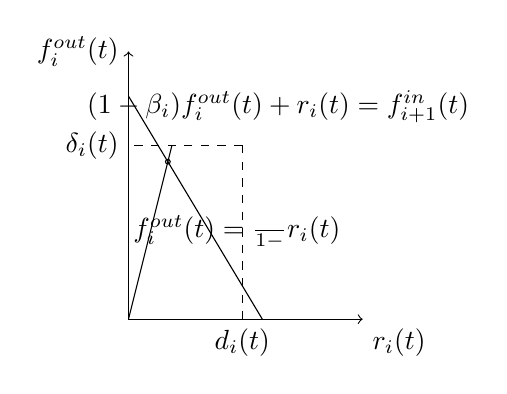
\begin{tikzpicture}[scale=1*.85,domain=0:1]

\def \rampDem{1.7}
\def \dem{2.6}
\def \priorityRat{0.8}
\def \splitRat{0.4}
\def \totalFlow{2}
\FontSmall


\coordinate (Z) at (0,0);
\coordinate (I1) at (\rampDem, 0);
\coordinate (I2) at (0, \dem);
\coordinate (I3) at (\rampDem, \dem);
\coordinate (A) at (0, {\totalFlow/(1-\splitRat)});
\coordinate (B) at (\totalFlow, 0);
\coordinate (C) at ({(1-\priorityRat)/\priorityRat*\dem}, \dem);

\draw[->] (Z) -- (3.5,0) node[below right]{$r_i(t)$};
\draw[->] (Z) -- (0,4) node[left]{$f^{\text{out}}_i(t)$};
\draw[dashed] (I3) -- (I1) node[below]{$d_i(t)$};
\draw[dashed] (I3) -- (I2) node[left]{$\delta_i(t)$};
\draw (A) -- (B) node[yshift=2.7cm, xshift=0.2cm]{$(1-\beta_i)f_i^{\text{out}}(t) + r_i(t) = f_{i+1}^{\text{in}}(t)$};
\draw (Z) -- (C) node[midway, xshift=1.1cm]{$f_i^{\text{out}}(t) = \frac{\priority{\icell}}{1-\priority{\icell}} r_i(t)$};
\draw (intersection of A--B and Z--C) circle (1pt);

\end{tikzpicture}
}
\label{fig:junctionFlowsInside}
}
\subfloat[Intersection outside the feasible set]{
\resizebox{.5\columnwidth}{!}{
	\input{TikZ/junctionFlowsOutside}
}
\label{fig:junctionFlowsOutside}
}
\caption{Junction flows given by the junction solver}
\label{fig:junctionFlows}
\end{figure}

%-----------------------------------------------------------------------------------------------------------------------------------------------------------------
\subsection{Riemann problem}

We consider a Riemann problem at junction $i$ and at time $t_0$, where the inputs are constant in time, and we look for a flux solution that is also constant in time (until the next shock), thus we will drop the dependency on time in the input flux and the junction fluxes. Since the fluxes are constant, we have $\frac{d}{dt} l_i(t) = \bar{D}_i - r_i$, therefore the buffer size grows linearly in time.


TODO: define a solution to the Riemann problem

%-----------------------------------------------------------------------------------------------------------------------------------------------------------------
\subsection{Self-similar solution}

At $t_0^+$, starting from the solution $(\bar{\rho}_i(t_0), \bar{\rho}_{i+1}(t_0))$ of the Riemann solver, we show that the flux solution to the junction solver are invariant,
\[
\js_{l_i(t_0^+)}(\bar{\rho}_i(t_0), \bar{\rho}_{i+1}(t_0)) = \js{l_i(t_0)}(\rho_i(t_0), \rho_{i+1}(t_0))
\]
and as a consequence, the solution of the Riemann solver is invariant
\[
\rs_{l_i(t_0^+)} (\bar{\rho}_i(t_0), \bar{\rho}_{i+1}(t_0)) = (\bar{\rho_i}(t_0), \bar{\rho}_{i+1}(t_0))
\]
In other words, we need to show that $r_i(t_0^+) = r_i(t_0)$, and $f_i^{\text{out}}(t_0^+) = f_i^{\text{out}}(t_0)$.


%-----------------------------------------------------------------------------------------------------------------------------------------------------------------
\subsubsection{Initially empty buffer}
We first consider the case where the buffer is initially empty, $l_i(t_0) = 0$, and the input flux is greater than the output flux, i.e.  $\bar{D}_i > r_i$, and the buffer is growing linearly. Thus $l_i(t_0^+) > 0$. From these assumptions, the onramp demand is given by
\begin{align*}
d_i(t_0) &= \min (u_i, r_i^{\max}, \bar{D}_i) \\
d_i(t_0^+) &= \min (u_i, r_i^{\max})
\end{align*}

\paragraph{Remark} We observe that the ramp demand at time $t_0^+$ can only increase, i.e.
\begin{equation}
d_i(t_0^+) \geq d_i(t_0)
\label{eq:buffer-rampDemandIncrease}
\end{equation}
since
\begin{align*}
d_i(t_0^+)
&= \min (u_i, r_i^{\max})\\
&\geq \min (u_i, r_i^{\max}, \bar{D}_i) \\
& =d_i(t_0)
\end{align*}
Moreover, if $r_i(t_0) = d_i(t_0)$, then we have equality $d_i(t_0^+) = d_i(t_0)$. Proof: since $r_i(t_0) = d_i(t_0) = \min (u_i, r_i^{\max}, \bar{D}_i)$ and $r_i(t_0) < \bar{D}_i$ (the buffer is growing), we necessarily have $\min (u_i, r_i^{\max}) < \bar{D}_i$, thus $\min(u_i, r_i^{\max}) = \min (u_i, r_i^{\max}, \bar{D}_i)$.

%------------------------------------------------------------------------------
\paragraph{Supply-constrained case}
First, we assume that the junction is supply-constrained at time $t_0$, i.e. $(1-\beta_i)\delta_i(t_0) + d_i(t_0) > \sigma_{i+1}(t_0)$. Therefore the mainline supply at time $t_0^+$ is
\begin{equation}
\sigma_{i+1}(t_0^+) = \sigma_{i+1}(t_0)
\label{eq:buffer-supplyIncrease}
\end{equation}

We consider three cases, depending on the flux solution of the junction solver.

\begin{figure}[h]
\centering
\subfloat[Solution on the boundary $r_i = d_i$]{
\resizebox{.33\columnwidth}{!}{
	\def \scale{1.5}
\begin{tikzpicture}[scale=\scale,domain=0:1]

\def \rampDem{1.7}
\def \dem{2.2}
\def \demPlus{2.5}
\def \priorityRat{0.2}
\def \splitRat{0.4}
\def \totalFlow{2.2}

\coordinate (Z) at (0,0);
\coordinate (I1) at (\rampDem, 0);
\coordinate (I2) at (0, \dem);
\coordinate (I2') at (0, \demPlus);
\coordinate (I3) at (\rampDem, \dem);
\coordinate (I3') at (\rampDem, \demPlus);
\coordinate (A) at (0, {\totalFlow/(1-\splitRat)});
\coordinate (B) at (\totalFlow, 0);
\coordinate (C) at ({(1-\priorityRat)/\priorityRat*\dem}, \dem);
\coordinate (D) at (intersection of A--B and Z--C);


\draw[->] (Z) -- (3.5,0) node[below right]{$r_i$};
\draw[->] (Z) -- (0,4) node[left]{$f^{\text{out}}_i$};

\draw (I3') -- (I1) node[below]{$d_i(t_0) = d_i(t_0^+)$};
\draw (I3') -- (I2') node[left]{$\delta_i(t_0^+)$};
\draw (A) -- (B) node[yshift=1cm, xshift=0cm]{};
\draw (Z) -- (D) node[midway, xshift=1cm]{};
\draw (intersection of A--B and I3--I1) circle (1pt) node[above right]{$(r_i(t_0^+), f_i^{\text{out}}(t_0^+))$};

\end{tikzpicture}
}
\label{fig:junctionBuffer-SupplyConstrained-Boundary1}
}
\subfloat[Solution on the boundary $f_i^{\text{out}} = \delta_i$]{
\resizebox{.33\columnwidth}{!}{
	% !TEX root = ../rampMeteringViaTheAdjoint.tex
\def \scale{1.5}
\begin{tikzpicture}[scale=\scale,domain=0:1]

\def \rampDem{1.7}
\def \rampDemPlus{2.0}
\def \dem{2.2}
\def \priorityRat{0.9}
\def \splitRat{0.4}
\def \totalFlow{2.2}

\coordinate (Z) at (0,0);
\coordinate (I1) at (\rampDem, 0);
\coordinate (I1') at (\rampDemPlus, 0);
\coordinate (I2) at (0, \dem);
\coordinate (I3) at (\rampDem, \dem);
\coordinate (I3') at (\rampDemPlus, \dem);
\coordinate (A) at (0, {\totalFlow/(1-\splitRat)});
\coordinate (B) at (\totalFlow, 0);
\coordinate (C) at ({(1-\priorityRat)/\priorityRat*\dem}, \dem);
\coordinate (D) at (intersection of A--B and Z--C);


\draw[->] (Z) -- (3.5,0) node[below right]{$r_i$};
\draw[->] (Z) -- (0,4) node[left]{$f^{\text{out}}_i$};

\draw[dashed] (I3) -- (I1) node[below left]{$d_i(t_0)$};
\draw (I3') -- (I1') node[below right]{$d_i(t_0^+)$};
\draw (I3') -- (I2) node[above left]{$\delta_i(t_0)$} node[below left]{$\delta_i(t_0^+)$};
\draw (A) -- (B) node[yshift=1cm, xshift=0cm]{};
\draw (Z) -- (D) node[midway, xshift=1cm]{};
\draw (intersection of A--B and I3--I2) circle (1pt) node[above right]{$(r_i(t_0^+), f_i^{\text{out}}(t_0^+))$};

\end{tikzpicture}
}
\label{fig:junctionBuffer-SupplyConstrained-Boundary2}
}
\subfloat[Solution in the interior of the feasible set]{
\resizebox{.33\columnwidth}{!}{
	% !TEX root = ../rampMeteringViaTheAdjoint.tex
\def \scale{1.5}
\begin{tikzpicture}[scale=\scale,domain=0:1]

\def \rampDem{1.7}
\def \rampDemPlus{2.0}
\def \dem{2.2}
\def \demPlus{2.5}
\def \priorityRat{0.6}
\def \splitRat{0.4}
\def \totalFlow{2.2}

\coordinate (Z) at (0,0);
\coordinate (I1) at (\rampDem, 0);
\coordinate (I1') at (\rampDemPlus, 0);
\coordinate (I2) at (0, \dem);
\coordinate (I2') at (0, \demPlus);
\coordinate (I3) at (\rampDem, \dem);
\coordinate (I3') at (\rampDemPlus, \demPlus);
\coordinate (A) at (0, {\totalFlow/(1-\splitRat)});
\coordinate (B) at (\totalFlow, 0);
\coordinate (C) at ({(1-\priorityRat)/\priorityRat*\dem}, \dem);
\coordinate (D) at (intersection of I2'--I3' and Z--C);


\draw[->] (Z) -- (3.5,0) node[below right]{$r_i$};
\draw[->] (Z) -- (0,4) node[left]{$f^{\text{out}}_i$};

\draw[dashed] (I3) -- (I1) node[below left]{$d_i(t_0)$};
\draw[dashed] (I3) -- (I2) node[left]{$\delta_i(t_0)$};
\draw (I3') -- (I1') node[below right]{$d_i(t_0^+)$};
\draw (I3') -- (I2') node[left]{$\delta_i(t_0^+)$};

\draw (A) -- (B) node[yshift=1cm, xshift=0cm]{};
\draw (Z) -- (D) node[midway, xshift=1cm]{};
\draw (intersection of A--B and Z--D) circle (1pt) node[below]{$(r_i(t_0^+), f_i^{\text{out}}(t_0^+))$};

\end{tikzpicture}
}
\label{fig:junctionBuffer-SupplyConstrained-Interior}
}
\caption{Self-similar solution in the case of a supply-constrained junction problem at time $t_0$}
\label{fig:junctionBuffer-SupplyConstrained}
\end{figure}


%------------------------------------------------------------------------------
\paragraph{(a)} The intersection is on the boundary of the feasible set
\[
r_i(t_0) = d_i(t_0)
\]
By the previous remark, we have
\begin{align*}
d_i(t_0) = d_i(t_0^+)
\end{align*}
The mainline demand can only increase $\delta_i(t_0^+) \geq \delta_i(t_0)$ (in fact $\delta_i(t_0^+) = f_i^{\max}$), and by~\eqref{eq:buffer-supplyIncrease}, $\sigma_{i+1}(t_0^+) = \sigma_{i+1}(t_0)$. Therefore we have
\begin{align*}
r_i(t_0) &= d_i(t_0^+) \\
f_i^{\text{out}}(t_0) &\leq \delta_i(t_0^+) \\
(1-\beta_1)f_i^{\text{out}}(t_0) + r_i(t_0) & \le \sigma_{i+1}(t_0^+)
\end{align*}
Therefore $(f_i^{\text{out}}(t_0), r_i(t_0))$ is a feasible point for the junction problem at time $t_0^+$, and is thus the unique solution (see Figure~\ref{fig:junctionBuffer-SupplyConstrained-Boundary1})


%------------------------------------------------------------------------------
\paragraph{(b)} The intersection is on the boundary of the feasible set
\[
f_i^{\text{out}}(t_0) = \delta_i(t_0)
\]
In this case the mainline demand is $\delta_i(t_0^+) = f_i^{\text{out}}(t_0)$, and by~\eqref{eq:buffer-rampDemandIncrease} and~\eqref{eq:buffer-supplyIncrease}
\begin{align*}
r_i(t_0) &\leq d_i(t_0^+) \\
f_i^{\text{out}}(t_0) &= \delta_i(t_0^+) \\
(1-\beta_1)f_i^{\text{out}}(t_0) + r_i(t_0) & < \sigma_{i+1}(t_0^+)
\end{align*}

Therefore $(f_i^{\text{out}}(t_0), r_i(t_0))$ is a feasible point for the junction problem at time $t_0^+$, and is thus the unique solution (see Figure~\ref{fig:junctionBuffer-SupplyConstrained-Boundary2})

%------------------------------------------------------------------------------
\paragraph{(c)} The intersection is strictly inside the feasible set

\begin{align*}
r_i(t_0) &< d_i(t_0) \\
f^{\text{out}}_i(t_0) &< \delta_i(t_0)
\end{align*}

The mainline demand is $\delta_i(t_0^+) = f_i^{\max}$. The ramp demand is $d_i(t_0^+) = \min (u_i, r_i^{\max}) \geq  \min (u_i, r_i^{\max}, \bar{D}_i) = d_i(t_0)$. Therefore we have
\begin{align*}
r_i(t_0) &< d_i(t_0^+) \\
f_i^{\text{out}}(t_0) &< \delta_i(t_0^+) \\
(1-\beta_1)f_i^{\text{out}}(t_0) + r_i(t_0) &< \sigma_{i+1}(t_0^+)
\end{align*}

Therefore $(f_i^{\text{out}}(t_0), r_i(t_0))$ is a feasible point for the junction problem at time $t_0^+$, and is thus the unique solution (see Figure~\ref{fig:junctionBuffer-SupplyConstrained-Interior})


%------------------------------------------------------------------------------
\paragraph{Demand-constrained case}
Now assume the junction is demand-constrained, i.e. $(1-\beta_i)\delta_i(t_0) + d_i(t_0) < \sigma_{i+1}(t_0)$. Then the feasible set contains a single point, and we have
\begin{align*}
f_i^{\text{out}}(t_0) &= \delta_i(t_0) \\
r_i(t_0) &= d_i(t_0)
\end{align*}

\begin{figure}[h]
\centering
\resizebox{.4\columnwidth}{!}{% !TEX root = ../rampMeteringViaTheAdjoint.tex
\def \scale{1.5}
\begin{tikzpicture}[scale=\scale,domain=0:1]

\def \rampDem{1.7}
\def \dem{2.2}
\def \priorityRat{0.7}
\def \splitRat{0.4}
\def \totalFlow{3.3}
\def \totalFlowPlus{4}

\coordinate (Z) at (0,0);
\coordinate (I1) at (\rampDem, 0);
\coordinate (I2) at (0, \dem);
\coordinate (I3) at (\rampDem, \dem);

\coordinate (A) at (0, {\totalFlow/(1-\splitRat)});
\coordinate (B) at (\totalFlow, 0);
\coordinate (A') at (0, {\totalFlowPlus/(1-\splitRat)});
\coordinate (B') at (\totalFlowPlus, 0);

\coordinate (C) at ({(1-\priorityRat)/\priorityRat*\dem}, \dem);
\coordinate (D) at (intersection of A'--B' and Z--C);
\coordinate (E) at (\rampDem, \dem);


\draw[->] (Z) -- (3.5,0) node[below right]{$r_i$};
\draw[->] (Z) -- (0,4) node[left]{$f^{\text{out}}_i$};

\draw (I3) -- (I1) node[below]{$d_i(t_0) = d_i(t_0^+)$};
\draw (I3) -- (I2) node[below left]{$\delta_i(t_0)$} node[above left]{$\delta_i(t_0^+)$};

\begin{scope}
\clip (Z) rectangle (3.5, 4);
\draw[dashed] (A) -- (B) node[midway, right]{$\sigma_{i+1}(t_0)$};
\draw (A') -- (B') node[midway, right]{$\sigma_{i+1}(t_0^+)$};
\end{scope}

\draw (Z) -- (D) node[midway, xshift=1cm]{};
\draw (E) circle (1pt) node[above]{$(r_i(t_0^+), f_i^{\text{out}}(t_0^+))$};

\end{tikzpicture}}
\caption{Self-similar solution in the case of a demand-constrained junction problem at time $t_0$}
\label{fig:junctionBuffer-DemandConstrained}
\end{figure}

At time $t_0^+$, the mainline demand is $\delta_i(t_0^+) = f_i^{\text{out}}(t_0)$, the ramp demand is $d_i(t_0^+) = d_i(t_0)$ (by the previous remark), and the supply can only increase, $\sigma_{i+1}(t_0^+) \geq \sigma_{i+1}(t_0)$. Therefore
\begin{align*}
r_i(t_0) &= d_i(t_0^+) \\
f_i^{\text{out}}(t_0) &= \delta_i(t_0^+) \\
(1-\beta_1)f_i^{\text{out}}(t_0) + r_i(t_0) &< \sigma_{i+1}(t_0^+)
\end{align*}
i.e. $(f_i^{\text{out}}(t_0), r_i(t_0))$ is a feasible point for the junction problem at time $t_0^+$, and is thus the unique solution (see Figure~\ref{fig:junctionBuffer-DemandConstrained})


%-----------------------------------------------------------------------------------------------------------------------------------------------------------------
\subsubsection{Initially non-empty buffer}





\subsection{Combined Section}\label{sub:bestselfsimilar}
% !TEX root = rampMeteringViaTheAdjoint.tex
This is an attempt to combine the work of the previous two main sections, as discussed the other day.
\paragraph{Definitions}
\begin{figure}
	\centering
	\begin{displaymath}
    \xymatrix{ \bullet \ar[r]| {\linkmlone} & \bullet   \ar[r]| {\linkmltwo} \ar[dr]| {\linkoff} & \bullet  \\
			    \ar[ur]|{\linkon}  &   &  }
\end{displaymath}
	\caption{Illustration of junction under consideration}
	\label{fig:contJuncIll}
\end{figure}
Parameters/Setup
\begin{itemize}
\item $\delta_{1}\left(\cdot\right),\sigma_{2}\left(\cdot\right),D,\beta,P,r^{\max}$
\item $I=\left\{ 1,r\right\} ,J=\left\{ 2\right\} $
\begin{itemize}
\item See Figure~\ref{fig:contJuncIll}
\end{itemize}
\end{itemize}
Max Flux
\begin{itemize}
\item $\gamma_{1,t}^{\max}=\delta_{1}\left(\rho_{1,t}\right),\gamma_{2,t}^{\max}=\sigma_{2}\left(\rho_{2,t}\right)$
\item $\gamma_{r,t}^{\max}=\begin{cases}
r^{\max} & l_{t}>0\\
\min\left(r^{\max},D\right) & \text{otherwise}
\end{cases}$
\item $\Gamma^{\max}\left(\rho_{1,t},\rho_{2,t},l_{t}\right)=$$\left(\gamma_{1,t}^{\max},\gamma_{2,t}^{\max},\gamma_{r,t}^{\max}\right)$
\item $\Omega_{i,t}=\left[0,\gamma_{i,t}^{\max}\right]$
\end{itemize}
Junction Problem
\begin{itemize}
\item $\mathcal{JS}\left(\gamma_{1}^{\max},\gamma_{2}^{\max},\gamma_{r}^{\max}\right)=\left(\gamma_{1},\gamma_{2},\gamma_{r}\right)$
is detailed in Section~\ref{sub:junction-model}
\end{itemize}
Mapping from fluxes to boundary densities
\begin{itemize}
\item $\psi_{1,t}\left(\gamma\right)=\rho_{1,t^{+}},\psi_{2,t}\left(\gamma\right)=\rho_{2,t^{+}}$
are described in Piccoli book
\item $\psi_{r,t}\left(\gamma\right)=l_{t^{+}}=l_t + \left(D-\gamma\right)\delta t$
\item $\Psi_{t}\left(\gamma_{1},\gamma_{2},\gamma_{r}\right)=\left(\psi_{i,t}\left(\gamma_{i}\right):i\in\left(1,2,r\right)\right)$
\end{itemize}
Riemann Solver
\begin{itemize}
\item $\mathcal{RS}\left(\rho_{1,t},\rho_{2,t},l_{t}\right)=\Psi\left(\mathcal{JS}\left(\Gamma^{\max}\left(\rho_{1,t},\rho_{2,t},l_{t}\right)\right)\right)=\left(\rho_{1,t^{+}},\rho_{2,t^{+}},l_{t^{+}}\right)$
\end{itemize}
Limiting Side: Whether demand or supply limits flux across junction
\begin{itemize}
\item $\mathcal{LS}_{t}=\begin{cases}
I & \gamma_{1,t}^{\max}\beta+\gamma_{r,t}^{\max}<\gamma_{2,t}^{\max}\\
J & \text{otherwise}
\end{cases}$
\item $\bar{\mathcal{LS}_{t}}=\begin{cases}
J & \gamma_{1,t}^{\max}\beta+\gamma_{r,t}^{\max}<\gamma_{2,t}^{\max}\\
I & \text{otherwise}
\end{cases}$
\end{itemize}
\textbf{Remark:} We do not consider the case where the queue instantaneously
goes from non-empty to empty. This would be the case where the initial shock and the emptying shock occur simultaneously, but this cannot be the case since there will always be a finite gap between the shocks, at which we could consider two separate Riemann problems.


\paragraph{Proof of self-similarity}
\begin{itemize}
\item $\gamma_{i}=\gamma_{i}^{\max}\implies\Omega_{i,0^{+}}=\Omega_{i,0}$

\begin{itemize}
\item For density links, this is a property of the $\psi$ mapping in Piccoli.
It is clear that the only time this may not be the case for the buffer
is when the buffer goes from empty to non-empty. But for this to be
the case, $D>r^{\max}=\gamma_{r,0}^{\max}$, therefore $\gamma_{r,0}^{\max}=\min\left(D,r^{\max}\right)=r^{\max}=\gamma_{r,0^{+}}^{\max}$.
\end{itemize}
\item $\forall i\in\mathcal{LS}_{0}\implies\Omega_{i,0^{+}}=\Omega_{i,0}$

\begin{itemize}
\item This follows from the property above and the properties of $\psi$.
\end{itemize}
\item $\forall i\in\bar{\mathcal{LS}}_{0}\implies\Omega_{i,0}\subseteq\Omega_{i,0^{+}}$

\begin{itemize}
\item For the density links, from the properties of $\psi$, when a link
is below its maximum flux, its maximum flux will only increase, i.e.
the upstream links become more congested, and the downstream links
become less congested. For the buffer, clearly $\forall D,r^{\max}:r^{\max}\ge\min\left(D,r^{\max}\right)$.
\end{itemize}
\item $\mathcal{LS}_{0^{+}}=\mathcal{LS}_{0}$

\begin{itemize}
\item This follows from the fact that the limiting side's feasible set remains
the same, while the non limiting side's feasible set only increases,
therefore the limiting side for time 0 will again be limiting for
$0^{+}$.
\end{itemize}
\item $\gamma_{i,0^{+}}=\gamma_{i,0}\forall i\in\left\{ 1,2,r\right\} \implies\mathcal{RS}$
is self similar

\begin{itemize}
\item From the properties of $\Psi$ and $\mathcal{JS}$, we have the property
that $\Psi_{t^{+}}\left(\gamma_{1,t},\gamma_{2,t},\gamma_{r,t}\right)=\left(\rho_{1,t^{+}},\rho_{2,t^{+}},\rho_{r,t^{+}}\right)$. Then we have:
\end{itemize}
\end{itemize}
\begin{eqnarray*}
\gamma_{0^{+}} & =\gamma_{0} & \implies\\
\rho_{0^{++}}=\Psi_{0^{+}}\left(\gamma_{0^{+}}\right)=\Psi_{0^{+}}\left(\gamma_{0}\right) & = & \rho_{0^{+}}
\end{eqnarray*}


\textbf{Theorem: }$\mathcal{RS}$ is self similar

\textbf{Proof:} We only need to show that $\gamma_{i,0^{+}}=\gamma_{i,0}\forall i\in\left\{ 1,2,r\right\} $.
When the problem is demand-limited, it is true from the fact that
the feasible set does not change for the limiting side (and the limiting
side does not change). When the problem is supply-limited, we have
that the incoming fluxes are determined by minimizing the distance of the incoming flux solution $\left(\gamma_{1},\gamma_{r}\right)$ from the intersection of $P$ line and the outgoing feasible set (Figure~\ref{fig:ssDistance}),
such that the total flux is maximized and feasible. Since the outgoing
feasible set and the $P$ value do not change, this intersection point
will not change between $t=0$ and $0^{+}$.

We consider the case when the intersection point occurs on the interior
of the incoming feasible set, and otherwise. For the first case, the
reference point is feasible, and thus reference point will be optimal
for both the original and final problem. See Figure~\ref{fig:virtualSSInteriorComb}.

Otherwise, exactly one of the incoming links $i\in\left\{ 1,r\right\} $
has $\gamma_{i,0}=\gamma_{i,0}^{\max}$, and the optimal point of
the problem at $t=0$ resides on the boundary of the feasible region.
Therefore $\Omega_{i,0}=\Omega_{i,0^{+}}$, and $\Omega_{j,0^{+}}\subseteq\Omega_{j,0}$,
where $j\in\left\{ 1,r\right\} \setminus\left\{ i\right\} $ is the
other incoming link. Therefore the flux solutions at time $t=0$ ($\gamma_0$) remain
feasible and on the boundary of the feasible set. Since our objective
is convex and the feasible set does not increase locally at $\gamma_{0}$,
the flux solution from $\mathcal{JS}$ at $t=0^{+}$ will equivalently
be $\gamma_{0}$. See Figure~\ref{fig:virtualSSBoundaryComb}.

For all initial data, we have demonstrated $\gamma_{i,0^{+}}=\gamma_{i,0}\forall i\in\left\{ 1,2,r\right\} $,
thus completing the proof.

\begin{figure}[h]
\centering
\subfloat[Minimizing distance from $P$ line]{
\resizebox{.33\columnwidth}{!}{
	% !TEX root = rampMeteringViaTheAdjoint.tex
\def \rampDem{1.7}
\def \dem{1.5}
\def \priorityRat{0.8}
\def \totalFlow{2.5}
\def \twoGap{.5}
\def \rulerOffset{.2}

\begin{tikzpicture}[scale=\scale,domain=0:1]

\coordinate (Z) at (0,0);
\coordinate (I1) at (\rampDem, 0);
\coordinate (I2) at (0, \dem);
\coordinate (I3) at (\rampDem, \dem);
\coordinate (I4) at (\rampDem+\twoGap, 0);
\coordinate (I5) at (\rampDem+\twoGap, \dem);
\coordinate (I6) at (0, \dem);
\coordinate (I7) at (\rampDem+\twoGap, \dem);
\coordinate (I8) at (\rampDem, \dem);
\coordinate (A) at (0, {\totalFlow});
\coordinate (B) at (\totalFlow, 0);
\coordinate (C) at ({(1-\priorityRat)/\priorityRat*\dem}, \dem);
\coordinate (D) at ({(1-\priorityRat)/\priorityRat*\dem*5}, \dem);
\coordinate (Cplus) at ({(1-\priorityRat)/\priorityRat*\totalFlow}, \totalFlow);
\coordinate (P1) at (intersection of I1--I3 and A--B);
\coordinate (P2) at (intersection of I2--I3 and A--B);
\coordinate (rulerOffset) at (\rulerOffset,\rulerOffset);


\draw[->] (Z) -- (3,0) node[below right]{$\gamma_{1,t}$};
\draw[->] (Z) -- (0,3) node[left]{$\gamma_{r,t}$};
\draw[dashed] (I8) -- (I1) node[below]{$\beta\gamma^{\max}_{1,t}$};
\draw[dashed] (I3) -- (I2) node[left]{$\gamma^{\max}_{r,t}$};
\draw (A) -- (B) node[left,yshift=.5cm]{$\gamma^{\max}_{2,0}=\beta\gamma_{1,t}+\gamma_{r,t}$};
\draw (Z) -- (C) node[below, xshift=1cm,yshift=-1cm,]{$\gamma_{1,t}=\frac{P}{1-P}\gamma_{r,t}$};
\draw[->,dashed] (C) -- (Cplus);
\draw[line width = 2pt] (intersection of A--B and Z--C) node (xseclabel){} circle (1.5pt);
\draw (intersection of A--B and Z--C) node [left](xseclabel2){$\left(P\gamma^{\max}_{2,t},\left(1-P\right)\gamma^{\max}_{2,t}\right)$};
\draw (intersection of I5--I2 and A--B) node (isectop) {};
\draw (intersection of I8--I1 and A--B) node (isecbottom) {};
\draw[line width = 3pt,|-|] (isectop) -- (isecbottom);
\draw[line width = 2pt] (intersection of A--B and Z--D) node (randcircle){} circle (1.5pt);
\draw (xseclabel) + (rulerOffset) node (off1) {};
\draw (randcircle) + (rulerOffset) node (off2) {};
\draw[color = red, line width = 2pt,<->] (off1) -- (off2) node[xshift=0cm,yshift=1cm] {Minimize};


\end{tikzpicture}

}
\label{fig:ssDistance}
}
\subfloat[Interior Example]{
\resizebox{.33\columnwidth}{!}{
	\def \rampDem{1.8}
\def \dem{2.5}
\def \priorityRat{0.55}
\def \totalFlow{3.2}
\def \twoGap{.5}
\def \twoGapDem{.3}


\begin{tikzpicture}[scale=\scale,domain=0:1]

\coordinate (Z) at (0,0);
\coordinate (I1) at (\rampDem, 0);
\coordinate (I2) at (0, \dem);
\coordinate (I3) at (\rampDem, \dem);
\coordinate (I4) at (\rampDem+\twoGap, 0);
\coordinate (I5) at (\rampDem+\twoGap, \dem);
\coordinate (I6) at (0, \dem+\twoGapDem);
\coordinate (I7) at (\rampDem+\twoGap, \dem+\twoGapDem);
\coordinate (I8) at (\rampDem, \dem+\twoGapDem);
\coordinate (A) at (0, {\totalFlow});
\coordinate (B) at (\totalFlow, 0);
\coordinate (C) at ({(1-\priorityRat)/\priorityRat*\dem}, \dem+\twoGapDem);
\coordinate (P1) at (intersection of I1--I3 and A--B);
\coordinate (P2) at (intersection of I2--I3 and A--B);


\draw[->] (Z) -- (4,0) node[below right]{$\gamma_{1,0^+}$};
\draw[->] (Z) -- (0,4) node[left]{$\gamma_{r,0^+}$};
\draw[dashed] (I8) -- (I1) node[below]{$\beta\gamma^{\max}_{1,0}$};
\draw[dashed, line width = 2pt] (I7) -- (I4) node[below]{$\beta\gamma^{\max}_{1,0^+}$};
\draw[dashed] (I5) -- (I2) node[left]{$\gamma^{\max}_{r,0}$};
\draw[dashed, line width = 2pt] (I7) -- (I6) node[left]{$\gamma^{\max}_{r,0^+}$};
\draw (A) -- (B) node{};
\draw[->] (Z) -- (C) node[above, xshift=1cm]{};
\draw[color=red, line width = 2pt] (intersection of A--B and Z--C) node[left] {Optimal} circle (1pt);


\end{tikzpicture}
}
\label{fig:virtualSSInteriorComb}
}
\subfloat[Boundary Example]{
\resizebox{.33\columnwidth}{!}{
	% !TEX root = rampMeteringViaTheAdjoint.tex
\def \rampDem{1.7}
\def \dem{1.5}
\def \priorityRat{0.8}
\def \totalFlow{2.5}
\def \twoGap{.5}

\begin{tikzpicture}[scale=\scale,domain=0:1]

\coordinate (Z) at (0,0);
\coordinate (I1) at (\rampDem, 0);
\coordinate (I2) at (0, \dem);
\coordinate (I3) at (\rampDem, \dem);
\coordinate (I4) at (\rampDem+\twoGap, 0);
\coordinate (I5) at (\rampDem+\twoGap, \dem);
\coordinate (I6) at (0, \dem);
\coordinate (I7) at (\rampDem+\twoGap, \dem);
\coordinate (I8) at (\rampDem, \dem);
\coordinate (A) at (0, {\totalFlow});
\coordinate (B) at (\totalFlow, 0);
\coordinate (C) at ({(1-\priorityRat)/\priorityRat*\dem}, \dem);
\coordinate (Cplus) at ({(1-\priorityRat)/\priorityRat*\totalFlow}, \totalFlow);
\coordinate (P1) at (intersection of I1--I3 and A--B);
\coordinate (P2) at (intersection of I2--I3 and A--B);


\draw[->] (Z) -- (3,0) node[below right]{$\gamma_{j,0^+}$};
\draw[->] (Z) -- (0,3) node[left]{$\gamma_{i,0^+}$};
\draw[dashed] (I8) -- (I1) node[below]{$\beta\gamma^{\max}_{j,0}$};
\draw[dashed, line width = 2pt] (I7) -- (I4) node[below]{$\beta\gamma^{\max}_{j,0^+}$};
\draw[dashed, line width = 2pt] (I5) -- (I2) node[left]{$\gamma^{\max}_{i,0},\gamma^{\max}_{i,0^+}$};
\draw (A) -- (B) node[yshift=1cm, xshift=0cm]{};
\draw (Z) -- (C) node[below, xshift=1cm,yshift=-1cm,]{};
\draw[dashed, ->] (C) -- (Cplus);
\draw (intersection of A--B and Z--C) node [right](xseclabel){} circle (1pt);
\draw[color=red, line width = 2pt] (intersection of I5--I2 and A--B) node[above,xshift=1cm] (optimallabel){Optimal} circle (1pt);

\end{tikzpicture}

}
\label{fig:virtualSSBoundaryComb}
}
\caption{Illustration of self-similar proof}
\label{fig:virtualSSFigureComb}
\end{figure}

